\documentclass[a4paper,11pt]{article}
\usepackage{amsmath,amsthm,amsfonts,amssymb,amscd,amstext,vmargin,graphics,graphicx,tabularx,multicol} 
\usepackage[francais]{babel}
\usepackage[utf8]{inputenc}  
\usepackage[T1]{fontenc} 
\usepackage{pstricks-add,tikz,tkz-tab,variations}
\usepackage[autolanguage,np]{numprint} 

\setmarginsrb{1.5cm}{0.5cm}{1cm}{0.5cm}{0cm}{0cm}{0cm}{0cm} %Gauche, haut, droite, haut
\newcounter{numexo}
\newcommand{\exo}[1]{\stepcounter{numexo}\noindent{\bf Exercice~\thenumexo} : \marginpar{\hfill /#1}}
\reversemarginpar


\newcounter{enumtabi}
\newcounter{enumtaba}
\newcommand{\q}{\stepcounter{enumtabi} \theenumtabi.  }
\newcommand{\qa}{\stepcounter{enumtaba} (\alph{enumtaba}) }
\newcommand{\initq}{\setcounter{enumtabi}{0}}
\newcommand{\initqa}{\setcounter{enumtaba}{0}}

\newcommand{\be}{\begin{enumerate}}
\newcommand{\ee}{\end{enumerate}}
\newcommand{\bi}{\begin{itemize}}
\newcommand{\ei}{\end{itemize}}
\newcommand{\bp}{\begin{pspicture*}}
\newcommand{\ep}{\end{pspicture*}}
\newcommand{\bt}{\begin{tabular}}
\newcommand{\et}{\end{tabular}}
\renewcommand{\tabularxcolumn}[1]{>{\centering}m{#1}} %(colonne m{} centrée, au lieu de p par défault) 
\newcommand{\tnl}{\tabularnewline}

\newcommand{\trait}{\noindent \rule{\linewidth}{0.2mm}}
\newcommand{\hs}[1]{\hspace{#1}}
\newcommand{\vs}[1]{\vspace{#1}}

\newcommand{\N}{\mathbb{N}}
\newcommand{\Z}{\mathbb{Z}}
\newcommand{\R}{\mathbb{R}}
\newcommand{\C}{\mathbb{C}}
\newcommand{\Dcal}{\mathcal{D}}
\newcommand{\Ccal}{\mathcal{C}}
\newcommand{\mc}{\mathcal}

\newcommand{\vect}[1]{\overrightarrow{#1}}
\newcommand{\ds}{\displaystyle}
\newcommand{\eq}{\quad \Leftrightarrow \quad}
\newcommand{\vecti}{\vec{\imath}}
\newcommand{\vectj}{\vec{\jmath}}
\newcommand{\Oij}{(O;\vec{\imath}, \vec{\jmath})}
\newcommand{\OIJ}{(O;I,J)}

\newcommand{\bmul}[1]{\begin{multicols}{#1}}
\newcommand{\emul}{\end{multicols}}

\newcommand{\reponse}[1][1]{%
\multido{}{#1}{\makebox[\linewidth]{\rule[0pt]{0pt}{20pt}\dotfill}
}}

\newcommand{\titre}[5] 
% #1: titre #2: haut gauche #3: bas gauche #4: haut droite #5: bas droite
{
\noindent #2 \hfill #4 \\
#3 \hfill #5

\vspace{-1.6cm}

\begin{center}\rule{6cm}{0.5mm}\end{center}
\vspace{0.2cm}
\begin{center}{\large{\textbf{#1}}}\end{center}
\begin{center}\rule{6cm}{0.5mm}\end{center}
}



\begin{document}
\pagestyle{empty}
\titre{Interrogation: Les angles}{Nom :}{Prénom :}{Classe}{Date}


\exo{2,5} Cours \\

\noindent \q Donner la définition des angles complémentaires.\\

\bmul{2}
\q Citer deux angles :\\
\qa alternes-internes ;\\
\qa correspondants ;\\
\qa opposés par le sommet ;\\
\qa supplémentaires.

\columnbreak

\begin{flushleft}
\includegraphics[scale=1]{COURS1.eps} 
\end{flushleft}


\emul


\exo{3} ABCD est un rectangle de centre O. Une droite (xy) qui passe par O coupe [AD] en un point E et [BC] en un point F.\\

\bmul{2}

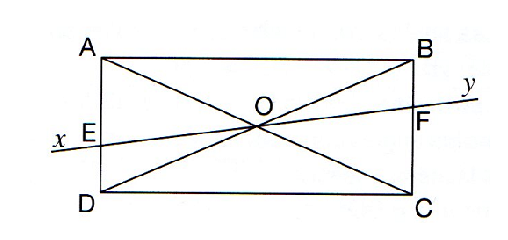
\includegraphics[scale=1]{cours.eps} 

\columnbreak

Compléter les phrases suivantes avec le vocabulaire du cours sur votre copie:\\
\initqa \qa $\widehat{ADO}$ et $\widehat{BOC}$ sont ...\\
\qa $\widehat{xED}$ et $\widehat{EFC}$ sont ...\\
\qa $\widehat{DAC}$ et $\widehat{ACB}$ sont ...\\
\qa $\widehat{CFO}$ et $\widehat{OFB}$ sont ...\\
\qa $\widehat{AEO}$ et $\widehat{OFC}$ sont ...\\
\qa $\widehat{DAC}$ et $\widehat{CAB}$ sont ...\\

\emul




\exo{3} Les droites (xy) et (tz)sont parallèles. La droite (uv) coupe (xy) en A et (tz) en B.\\

\bmul{2}

\initq \q On cherche la mesure de l'angle $\widehat{tBu}$. Rédiger une \textbf{démonstration} qui permette de trouver cette mesure.\\
\begin{center}
\includegraphics[scale=1]{DEM.eps} 
\end{center}

\columnbreak

\q On cherche à nouveau la mesure de l'angle $\widehat{tBu}$. Rédiger une \textbf{démonstration} qui permette de trouver cette mesure.\\
\begin{center}
\includegraphics[scale=1]{dem1.eps} 
\end{center}

\emul



\exo{1,5} Les droites (d) et (d') sont-elles parallèles ? Pour répondre à cette question vous rédigerez une \textbf{démonstration} .

\begin{center}
\includegraphics[scale=1]{dtepara.eps} 
\end{center}


\end{document}
